\section{Schwingungen}
\subsection{Freie Schwingung}
\bsp{Beispiel}

\begin{minipage}{0.47\textwidth}
    Feder~-~Dämpfer~-~System.
    
    Eine Masse $m$ hängt an einer Feder und ist
    an einen Flüssig-Dämpfer angeschlossen.
\end{minipage}
\begin{minipage}[r]{0.49\textwidth}
    \hfill
    \begin{circuitikz}
        \draw (-1,0) -- (1,0);
        \foreach \x in {-9,...,9}
            \draw ( {(\x-1)/10}, 0.1 ) -- ({\x/10},0);
        \coordinate (mass) at (0,-1.7);
        \draw (0,0) to [L] (mass) ;
        \node at (0,-1) [right,xshift=0.2cm] {Federkonstante $k$} ;
        \fill (mass) circle [radius=0.2] node[left,xshift=-0.1cm] {$m$};
        \draw (mass) -- (0,-3) -- + (0.5,0) -- + (-0.5,0);
        \draw (-1,-2.5) -- ++ (0,-1) -- ++ (2,0) -- ++ (0,1);
        \draw[decorate,decoration=snake] (-1, -2.7) -- ++ (2,0);
        \node[right] at (1,-3) {Dämpfer $r$};
        \draw[->] (-1.5,-3) -- ++ (0,2.5) node[midway,left] {$x$};
    \end{circuitikz}
\end{minipage}

DGL: $F=a\cdot m = -k\cdot x-r\cdot \dot{x}$
\begin{equation*}
\boxed{\ddot{x} + \frac{r}{m}\cdot\dot{x}+\frac{k}{m}\cdot x=0}
\end{equation*}
Freie, gedämpfte Schwingung

Lösung:
\begin{equation*}
    \ddot{x} + \underbrace{\frac{r}{m}}_{2\delta}\cdot\dot{x}+
    \underbrace{\frac{k}{m}}_{\omega_0^2}\cdot x=0
\end{equation*}
\begin{eqnarr}
    \delta^2 - \omega_0^2 &=&  \left( \frac{r}{2m} \right)^2-\frac{k}{m}\\
    &>& 0 \Rightarrow \text{Fall 1 (Kriechfall)} \\
    &=& 0 \Rightarrow \text{Fall 2 (aperiodischer Grenzfall)} \\
    &<& 0 \Rightarrow \text{Fall 3 (Schwingungsfall)} \\
\end{eqnarr}

\subsection*{a) Starke Dämpfung (Kriechfall)}
\begin{equation*}
    \boxed{\delta>\omega_0}
\end{equation*}
\begin{equation*}
    \lambda_{1,2} = -\delta\pm\underbrace{\sqrt{\delta^2-\omega_0^2}}_
    {>0 \text{ und }<\delta}<0
\end{equation*}
Lösung: \begin{equation*}
    x(t) = C_1\cdot e^{\lambda_1\cdot t} + C_2\cdot e^{\lambda_2\cdot t}
\end{equation*}

\subsection*{b) Aperiodischer Grenzfall}
\begin{equation*}
    \boxed{\delta=\omega_0}
\end{equation*}
\begin{equation*}
    \lambda = -\delta
\end{equation*}
Lösung: \begin{equation*}
    x(t) = C_1\cdot e^{-\delta\cdot t} + C_2\cdot t\cdot e^{-\delta\cdot t}
\end{equation*}

\subsection*{c) Schwache Dämpfung}
\begin{equation*}
    \boxed{\delta<\omega_0}
\end{equation*}
\begin{equation*}
    \omega_d = \sqrt{\omega_0^2-\delta^2}<\omega_0
\end{equation*}
Lösung: \begin{eqnarr}
    x(t)&=&  e^{-\delta \cdot t}\cdot \left[
        C_1\cdot\sin(\omega_d \cdot t) +
        C_2\cdot\cos(\omega_d \cdot t) 
        \right]\\
        &=& C\cdot e^{-\delta \cdot t} \cdot
        \sin\left( \omega_d\cdot t+\phi_d \right)\\
        &=& C\cdot e^{-\delta \cdot t} \cdot
        \cos\left( \omega_d\cdot t+\varphi_d \right)
\end{eqnarr}

%%%%%%%%%%%%%%%%%%%%%%%%%%%%%%%%%%%%%%%%%%%%%
\subsection{Erzwungene Schwingung}
Erzwungene Schwingung bedeutet:
\begin{outline}
    \1 Schwach gedämpftes System ($\delta<\omega_0$)
    \1 Periodische Erregung
\end{outline}
\begin{eqnarr}
    m\cdot \ddot{x}+r\cdot\dot{x}+k\cdot x&=& F_0\cdot\sin( \omega t)\\
    \ddot{x}+\underbrace{\frac{r}{m}}_{2\delta} \cdot\dot{x}
                  +\underbrace{\frac{k}{m}}_{\omega_0^2}\cdot x
                  &=& \underbrace{\frac{F_0}{m}}_{k_0}\cdot\sin( \omega t)\\
\end{eqnarr}

Lösung:
\begin{eqnarr}
x(t) &=&  x_h+x_p \\
&=& e^{-\delta t}\left(
    C_1\sin\left( \omega_d t \right)+C_2\cos\left( \omega_d t \right)
\right)
    +A \sin\left( \omega t-\varphi \right)
\end{eqnarr}

Was passiert wenn $t\rightarrow \infty$?
\begin{equation*}
    x(t) = \underbrace{e^{-\delta t}\left(
        C_1\sin\left( \omega_d t \right)+C_2\cos\left( \omega_d t \right)
\right)
    }_{\rightarrow 0}
    +A \sin\left( \omega t+\varphi \right)
\end{equation*}

Die stationäre Lösung ist 
\begin{equation*}
    \boxed{x_p = A\cdot \sin(\omega t - \varphi)}
\end{equation*}

\begin{outline}
    \1[] $A=A(\omega,\omega_0,\delta)$: \underline{Amplitudengang}
    \1[] $\varphi=\varphi(\omega,\omega_0,\delta)$: \underline{Phasengang}
\end{outline}

Bestimmen von $A$ und $\varphi$: Komplex rechnen mit 
\begin{eqnarr}
    \underline{K}(t) &=& K_0 e^{j\omega t}\\
    \underline{x}(t) &=& A e^{j(\omega t-\varphi)}\\
    \Rightarrow &&\\
    K(t) &=& \text{Im }\underline{K}(t)\\
    x_p(t) &=& \text{Im }\underline{x}(t)\\
\end{eqnarr}
In DGL einsetzen
\begin{eqnarr}
    \underline{x}(t) &=& A e^{j(\omega t-\varphi)}\\
    \dot{\underline{x}}(t) &=& j\omega A e^{j(\omega t-\varphi)}\\
    \ddot{\underline{x}}(t) &=& -\omega ^2 A e^{j(\omega t-\varphi)}\\
\end{eqnarr}

\begin{eqnarr}
    -\omega ^2 A e^{j(\omega t-\varphi)}
    +2\delta j\omega A e^{j(\omega t-\varphi)}
    +\omega_0^2 A e^{j(\omega t-\varphi)} 
    &=& K_0 e^{j\omega t}\\
    -\omega ^2 A 
    +2\delta j\omega A
    +\omega_0^2 A 
    &=& K_0 e^{-j(\omega t-\varphi)} e^{j\omega t}\\
    -\omega^2A +2\delta j\omega A +\omega_0^2 A  &=& K_0  e^{j\varphi}\\
    \omega_0^2 -\omega^2 +j (2\delta \omega) 
        &=& \frac{K_0}{A}  e^{j\varphi}\\
\end{eqnarr}
\begin{center}
    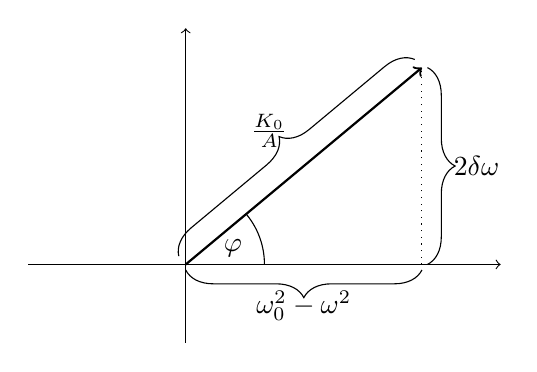
\begin{tikzpicture}
        \draw (-2,0) -- (0,0) -- (0,-1);
        \draw[<->] (0,3) -- (0,0) -- (4,0);

        \draw[->,thick] (0,0) -- (3,2.5);
        \draw[decorate,decoration={brace,amplitude=10pt},yshift=3pt,xshift=-2.5pt]
        (0,0) -- (3,2.5) node [midway,above left] {$\frac{K_0}{A}$};
        \draw[decorate,decoration={brace,mirror,amplitude=10pt},yshift=-2pt]
        (0,0) -- (3,0) node [midway,below,yshift=-4pt] {$\omega_0^2-\omega^2$};
        \draw[decorate,decoration={brace,mirror,amplitude=10pt},xshift=2pt]
        (3,0) -- (3,2.5) node [midway,right,xshift=6pt] {$2\delta\omega$};
        \draw[dotted] (3,0) -- (3,2.5) ;
        \node at (0.6,0.2) {$\varphi$};
        \clip (0,0) -- (3,0) -- (3,2.5) -- (0,0);
        \draw (0,0) circle[radius =1];
    \end{tikzpicture}
\end{center}
Pythagoras
\begin{equation*}
    \frac{K_0^2}{A^2} = \left( \omega_0^2 -\omega^2 \right)^2+4\delta^2\omega^2
\end{equation*}
$\Rightarrow$
\begin{equation*}
    \boxed{
        A = \frac{K_0}
        {\sqrt{\left( \omega_0^2-\omega^2 \right)^2+4\delta^2\omega^2}}
    }
\end{equation*}
